\chapter{Background}
This chapter explains the methods and concepts these are seperated in 2 parts one for basic knowledge and 

\section{Basic Knowledge}
Important knowledge for the contents of the thesis mainly the what translation, automatic Speech recognition and dropout


\subsection{Automatic Speech Recognition}
Automatic speech recognition systems or short ASR systems are systems that recognise and transcribe spoken language. 
%TODO

\subsection{Translation}
Translation is the practice of translating text or language from one language into another language. This can be done by hand by a human or in a very statical approach where a dictionary is used to directly translate the text 
%TODO
\subsubsection{Speech translation}
Speech translation or spoken language translation is simmilar to the regular translation but it has, like the name says, spoken language as the basis instead of text. 
%TODO


\subsection{Dropout}
- has been utilised in DNN to measure uncertainty
- mainly in Deep architectures but also in Auto-encoders
-in ASR it has been tried here  \cite{8683086}
- in ASR it mainly stems from noisy audio 
%TODO


\subsection{Transcription probability}
the probability that the ASR component transcribes the audio to this sequence of text
%TODO


\subsection{Translation probability}
- the probability that the model generates the sequence $y = y_1, y_2 \dots y_n$ for the input $x=x_1, x_2 \dots x_n$
norm the translation probabilty over the length of the transcribed and translation 
%TODO
\subsection{Pearsoncorrelation}
method to see how correlated 2 sets of values are
is 1 if it's correlated and -1 if it's inversely correlated 
if it's 0 the sets are not correlated at all
%TODO

\section{Models}
\subsection{Decoder-Encoder}
-Encoder-Decoder Models are Models that contain a Encoder, lorem ypsum 
and a Decoder, lorem ypsum
-the encoder output is then used as input for the decoder that produces the output of the model 
-Encoder-Decoder Achitecture is used for Sequence-to-Sequence models esp. more complex/advanced Sequence-to-Sequence models 
%TODO expand, add gaphics add citations 

\subsection{Transformer}
Neural Network architecture that was first introduced in the paper Attention is all you need \cite{vaswani2023attentionneed} that makes use of selfattention mechanisms. it has a Encoder-Decoder structure
%TODO

\subsection{ Cascaded Models}
Cascaded Speech translation Models consist of 2 parts a part that is resposnibe for transcribing the audio, which is usually done with an ASR model, and a part that is responisble for translating the resulting transcription, which is done with neural machine translation or statistical machine translation. 
%TODO citation and expand
\subsection{End-to-End Models}
End-to-End Speech translation models do not have the explicit split between the Automatic Speech Recognition model and the translation, this means that such a model gets audio as an input and outputs the text in the target language. 
%TODO citations, different architectures and expand
\subsection{Whisper}
Whisper is a multilingual multitask Model that is focused on speech processing and was proposes in the Robust Speech Recogintion via Large-Scale Weak Supervsion paper \cite{radford2022robust} 
%TODO
\subsection{Seamless}
Seamless is a Multimodal model that uses a Transformer architecture. 
the architecture was proposed in \cite{seamless2023}Read Aloud: A Text to Speech Voice Reader 
%TODO

\subsection{DeltaLM}
DeltaLM is one of the current state of the art Neural Machine Translation models and the architectures that was proposed in \cite{ma2021deltalm}. It is based off of the classical Encoder-Decoder structure but both the encoder and decoder are initialised with the pretrained multilingual encoder. The training happens in a self-supervised manner. 

In addition to this is the Decoder a Interleaved Transformer Decoder, which is not the same architecture as the encoder and differs from the standard Transformer decoder in that the Transformerblocks now consist of a self-attention layer, two feed-forward networks and a cross-attention layer which are arranged as seen in \ref{fig:interleaved decoder}. 
This way of building the decoder is more similar to the structure of the encoder and makes it easier to leverage the pretrained encoder. The interleaved decoder is then initialised with the layers from the pretrained encoder, which is the InfoXLM \cite{chi2021infoxlminformationtheoreticframeworkcrosslingual}, in the following way, the self-attention and the bottom FFN layers are initialised wiht the odd layers of the InfoXLM encoder and the cross-attention and top FFN layers are initialised with the even layers. 

\begin{figure}
    \centering
    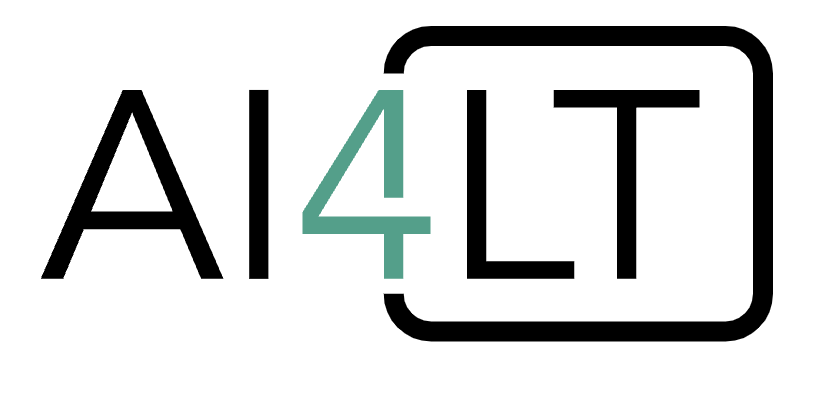
\includegraphics[width=0.5\linewidth]{Latex/logos/AI4LT_logo.png}
    \caption{Vanilla Transformer Decoder (left) compared to the interleaved Transformer decoder(right)}
    \label{fig:interleaved decoder}
\end{figure}
%TODO
